\documentclass[conference]{IEEEtran}
\IEEEoverridecommandlockouts

\usepackage{cite}
\usepackage{amsmath,amssymb,amsfonts}
\usepackage{algorithm}
\usepackage{algorithmic}
\usepackage{graphicx}
\usepackage{pifont}
\usepackage{makecell}
\usepackage{textcomp}
\usepackage{xcolor}
\usepackage{booktabs}
\usepackage{multirow}
\usepackage{array}
\usepackage{hyperref}
\usepackage{amsthm}
\usepackage{tikz}
\usetikzlibrary{positioning,arrows.meta,shapes.geometric,fit,backgrounds,calc}
\theoremstyle{definition}
\newtheorem{proposition}{Proposition}
\newcommand{\cmark}{\ding{51}}
\newcommand{\xmark}{\ding{55}}

% Override IEEEtran's default ALL-CAPS table captions; render in sentence case per IEEE style.
\usepackage[compatibility=false]{caption}
\captionsetup[table]{singlelinecheck=false, font=footnotesize, labelfont={sc}, textfont=normalfont}

\def\BibTeX{{\rm B\kern-.05em{\sc i\kern-.05em b}\kern-.05em\TeX}}

\begin{document}

\title{Intent-Adaptive Hybrid Retrieval and Heterogeneous-Space Person Fusion for Conversational Video Surveillance}

\author{\IEEEauthorblockN{Sujal M H\IEEEauthorrefmark{1},
Sujnan Kumar\IEEEauthorrefmark{1},
Yashas Shetty\IEEEauthorrefmark{1},
Suhan D Shet\IEEEauthorrefmark{1},
and Ravinarayana B\IEEEauthorrefmark{2}}
\IEEEauthorblockA{\IEEEauthorrefmark{1}Department of Computer Science \& Engineering, \\
Mangalore Institute of Technology \& Engineering, Moodabidre, India \\
\IEEEauthorrefmark{2}Head, Department of Computer Science \& Engineering, \\
Mangalore Institute of Technology \& Engineering, Moodabidre, India \\
Email: \{sujalmh9, sujnankumar439, yashass825, suhanshet2004\}@gmail.com, hodcse@mite.ac.in}}

\maketitle

\begin{abstract}
Hybrid retrieval over surveillance video typically combines a structured metadata filter with a dense semantic index using a \emph{fixed} mixing weight, which catastrophically mis-ranks counting and action queries. We make three novel contributions that, in combination, raise mean Precision@5 (macro-averaged over five query categories) on a 150-query natural-language benchmark from 0.67 (best fixed-$\alpha$ baseline, $\alpha{=}0.3$) to 0.83. \textbf{(C1)} An \emph{intent-adaptive blending function} $\alpha(F,\iota,n_s,n_v)$ that produces a closed-form, per-query mixing weight from the parsed filter $F$, the predicted query intent $\iota$, and the structured/semantic result-set imbalance, with two hard overrides for counting and action queries (Eq.~\eqref{eq:adaptive_alpha}); we show (under empirical concavity assumptions) why fixed-$\alpha$ schemes cannot match the per-category optima simultaneously. \textbf{(C2)} A \emph{heterogeneous-space person descriptor} that fuses a SigLIP visual embedding ($\mathbb{R}^{768}$) and a Sentence-Transformers attribute-text embedding ($\mathbb{R}^{384}$) into a single L2-normalized $\mathbb{R}^{1152}$ vector by weighted concatenation rather than the naive same-space addition used by prior multimodal Re-ID work; an ablation shows a 10.7-pp F$_1$ gain over the best unimodal index and a 2.2-pp gain over a same-space late-fusion variant. \textbf{(C3)} A \emph{conversational alert grammar} that reuses the same structured-output LLM parser to materialize fully-typed alert rules (event, object, zone, time, severity, cooldown, side-effects) from free-text utterances, eliminating manual rule authoring; we report 91\% rule-correctness on a held-out alert-authoring benchmark. The contributions are deployed inside a nine-model real-time pipeline that sustains 2~FPS per camera over a 4-camera deployment with a 109~ms median FAISS lookup over 312k indexed person descriptors.
\end{abstract}

\begin{IEEEkeywords}
Hybrid Retrieval, Intent-Adaptive Ranking, Multimodal Person Re-ID, Heterogeneous Embedding Fusion, Conversational Alert Authoring, Vision--Language Surveillance, Natural Language Querying.
\end{IEEEkeywords}

\section{Introduction}

\IEEEPARstart{N}{atural}-language interfaces over surveillance video are now technically feasible: instance segmentation, person Re-ID, and contrastive vision--language models are mature, and structured-output LLMs can convert a user utterance into a typed query schema. The unsolved problem is \emph{how to rank} the resulting candidate frames: a structured filter (\textit{``persons in Zone~A between 22:00 and 23:00''}) and a semantic vector lookup (\textit{``red jacket loitering near the entrance''}) produce two incommensurable score scales. The dominant fusion strategies in the literature are a fixed convex sum $\alpha S_{\text{struct}} + (1-\alpha) S_{\text{sem}}$ tuned once per system~\cite{b7,b11,b12,b29}, parameter-free Reciprocal Rank Fusion~\cite{b27}, or sequential filter-then-rank pipelines~\cite{b30}. We show empirically (Table~\ref{tab:alpha_baseline}) that no single $\alpha$ simultaneously serves counting, finding, tracking, and action queries: a fixed $\alpha=0.5$ collapses to 0.18~P@5 on action queries and a fixed $\alpha=1.0$ collapses to 0.04~P@5 on find queries, while no fixed value exceeds 0.67 macro-mean P@5 across all five categories.

A second open problem is the per-person descriptor. Prior multimodal person Re-ID work~\cite{b22b,b32,b33,b34,b35} either fuses two same-space embeddings by addition or trains a joint dual encoder, both of which require either dimension-matched backbones or a dataset for joint contrastive training that surveillance deployments rarely have.

A third open problem is rule authoring: existing alert engines (Verkada Command, Avigilon Unity, BriefCam Investigator) require an IT operator to translate a behavioral description into a typed rule, a productivity bottleneck that limits the number of useful rules in a deployment.

\subsection*{Contributions}
\begin{enumerate}
\item \textbf{Intent-adaptive hybrid retrieval} (\S\ref{sec:adaptive_alpha}). A closed-form, training-free mixing function $\alpha(F,\iota,n_s,n_v)$ with two hard overrides; an override-gap argument (Proposition~\ref{lem:mono}) under empirical concavity; +0.16 macro-mean P@5 over the best fixed-$\alpha$ baseline.
\item \textbf{Heterogeneous-space person fusion} (\S\ref{sec:fusion}). A weighted-concatenation descriptor that fuses backbones of incompatible dimensionality without joint training; +10.7-pp F$_1$@10 over the strongest unimodal index, +2.2-pp over a same-space late-fusion baseline.
\item \textbf{Conversational alert authoring} (\S\ref{sec:alert_grammar}). A typed grammar reusing the query parser; 91\% full-rule correctness (all 9 fields including cooldown and cadence) on a 60-utterance held-out benchmark.
\item \textbf{An end-to-end open implementation} validating all three contributions on a 4-camera live deployment (\S\ref{sec:eval}).\footnote{Code: \url{https://github.com/sujalmh/intent-adaptive-hybrid-surveillance} (to be released upon acceptance).}
\end{enumerate}

\section{Related Work and Position}

We compare directly with the closest published work along the three contribution axes (Table~\ref{tab:related}).

\textbf{Hybrid structured/semantic retrieval.} Combining dense and sparse / structured retrieval is established practice in IR~\cite{b25,b27,b29}, with two dominant fusion strategies: weighted convex combination of normalized scores (a single fixed $\alpha$~\cite{b29}) and parameter-free Reciprocal Rank Fusion~\cite{b27}. Query-dependent weighting itself is not new in IR -- learning-to-rank and query-dependent fusion have long adapted weights to query features -- but those approaches typically (i)~learn weights from large-scale click data, (ii)~operate on text-only sparse/dense pairs, and (iii)~lack hard overrides for semantically infeasible branches. The closest recent analogues, HyST~\cite{b30} (sequential LLM-filter then dense) and Agentic-RAG~\cite{b3} (router-based re-routing), still do not produce a per-query blended score. Forensic-search systems for surveillance video (VIDEX~\cite{b7}, three-stage DL~\cite{b12}, object-based IR~\cite{b11}) and CLIP+RAG pipelines~\cite{b1,b19} use a single retrieval branch (typically dense CLIP) without a structured-filter complement. We are not aware of prior work in the surveillance-video setting that computes the mixing weight per-query from parsed intent and result-set evidence with category hard overrides; the contribution here is the specific surveillance-tailored instantiation rather than the general idea of query-adaptive weighting.

\textbf{Multimodal person Re-ID.} Heterogeneous-dimensional concatenation of frozen encoders is itself a known retrieval pattern (e.g., in retrieval-augmented generation~\cite{b4} and general multimodal IR), so we do not claim the construction is new in IR at large. What we claim is its use as the \emph{primary} person descriptor in surveillance Re-ID: prior NL-based person-search work (CUHK-PEDES~\cite{b32}, CLIP-ReID~\cite{b33}, image-text modal fusion~\cite{b34}, TriReID~\cite{b35}) couples a dual encoder either by joint contrastive training or by descriptive-fusion modules over modalities of the \emph{same} dimensionality, while same-space late-fusion baselines such as RRF~\cite{b27} require dimension-matched encoders or two independent indices. We are not aware of a surveillance Re-ID system that uses weighted concatenation of heterogeneous frozen encoders as a single FAISS index, with the mixing weights calibrated on as few as 50 labeled pairs.

\textbf{Conversational alert authoring.} Existing surveillance products~\cite{b7,b8,b12} expose form-driven rule editors, and structured-output LLMs~\cite{b20} are by now standard for slot-filling and tool-use; the novelty we claim is the specific reuse of the same query-parsing schema to materialize a 9-tuple typed alert rule end-to-end, rather than a fundamentally new LLM capability. We are not aware of a published surveillance system that exposes this combined query/alert authoring path.

Generic deep-learning components (YOLO~\cite{b13,b14}, BoT-SORT~\cite{b22}, OSNet~\cite{b22b}, OpenCLIP~\cite{b18,b18b}, SigLIP~\cite{b24}, MiniLM~\cite{b23}, Qwen2-VL~\cite{b17}, OpenVINO PAR~\cite{b15}, FAISS~\cite{b25}, MMR~\cite{b26}) are used as off-the-shelf building blocks and are not claimed as contributions; we summarize their roles in Table~\ref{tab:models} and direct the reader to the cited work for their internals.

\begin{table}[!t]
\caption{Position relative to closest related work along the three novel axes; entries indicate the kind of mechanism used.}
\label{tab:related}
\centering
\scriptsize
\setlength{\tabcolsep}{3pt}
\begin{tabular}{@{}p{2.6cm}p{1.25cm}p{1.45cm}p{1.05cm}@{}}
\toprule
System / Work & \makecell[l]{Per-query\\ adapt.\ $\alpha$} & \makecell[l]{Heterog.-sp.\\ Re-ID fusion} & \makecell[l]{Conv.\ alert\\ authoring} \\
\midrule
Fixed-$\alpha$ hybrid~\cite{b29}     & fixed       & ---            & --- \\
RRF~\cite{b27}                        & rank-only   & rank-only      & --- \\
HyST~\cite{b30}                       & sequential  & ---            & --- \\
Agentic RAG~\cite{b3}                 & route-only  & ---            & --- \\
VIDEX~\cite{b7}                       & \xmark      & \xmark         & \xmark \\
3-Stage DL~\cite{b12}                 & \xmark      & \xmark         & \xmark \\
Object-IR~\cite{b11}                  & \xmark      & \xmark         & \xmark \\
LLM-Surv.~\cite{b1}                   & \xmark      & \xmark         & \xmark \\
CUHK-PEDES~\cite{b32}                 & ---         & joint-trained  & --- \\
CLIP-ReID~\cite{b33}                  & ---         & joint-trained  & --- \\
Img-Txt Fusion~\cite{b34}             & ---         & same-space     & --- \\
TriReID~\cite{b35}                    & ---         & same-space     & --- \\
OSNet~\cite{b22b}                     & ---         & visual-only    & --- \\
SigLIP/CLIP~\cite{b24}                & ---         & same-space     & --- \\
\textbf{This work}                    & \cmark      & \cmark         & \cmark \\
\bottomrule
\end{tabular}
\end{table}

\section{Background and System Substrate}

The novel contributions are deployed inside a nine-model real-time pipeline. We summarize it here for self-containedness; component internals are deferred to the cited references and to the open implementation. Live RTSP / MJPEG streams (1080p, 2~FPS) and uploaded video files are processed by YOLOv11m-seg~\cite{b14} for instance segmentation, BoT-SORT~\cite{b22} with OSNet $x1\_0$~\cite{b22b} for multi-object tracking and Re-ID, the OpenVINO PAR-crossroad-0238~\cite{b15} model for seven multi-label person attributes (sigmoid output), and a histogram-based dominant-color estimator on a quantized CIE~LAB grid with CIEDE2000~\cite{b16} nearest-neighbor naming over a 25-class CSS3 palette. Two FAISS \texttt{IndexFlatIP} indices~\cite{b25} hold the resulting embeddings: a scene index ($\mathbb{R}^{512}$, OpenCLIP ViT-B/32~\cite{b18b}) and a person index ($\mathbb{R}^{1152}$, our novel descriptor of \S\ref{sec:fusion}). MongoDB stores 13 compound-indexed collections of structured detection metadata. A FastAPI backend exposes 30+ REST endpoints to a Next.js dashboard. Frame captions come from a tiered VLM pipeline (Qwen2-VL-2B-Instruct~\cite{b17} with ViT-GPT2 and zero-shot CLIP fallbacks~\cite{b18,b18b,b19}). The natural-language parser is a structured-output LLM (GPT-4o-mini~\cite{b20} by default; configurable to local Ollama).

\begin{table}[!t]
\caption{Off-the-shelf components and their roles. None are claimed as contributions.}
\label{tab:models}
\centering
\footnotesize
\begin{tabular}{@{}lll@{}}
\toprule
Component & Role & Output \\
\midrule
YOLOv11m-seg~\cite{b14}     & Detection + masks       & per-frame \\
BoT-SORT~\cite{b22}          & MOT association         & track IDs \\
OSNet $x1\_0$~\cite{b22b}    & Re-ID appearance        & 512-d \\
PAR-crossroad-0238~\cite{b15}& Person attributes       & 7-d (sigmoid) \\
OpenCLIP ViT-B/32~\cite{b18b}& Scene embedding         & 512-d \\
SigLIP-base-p16~\cite{b24}   & Person visual           & 768-d \\
MiniLM-L12-v2~\cite{b23}     & Attribute text          & 384-d \\
Qwen2-VL-2B~\cite{b17}       & Captioning              & text \\
GPT-4o-mini~\cite{b20}       & NL parsing              & JSON \\
\bottomrule
\end{tabular}
\end{table}

\section{C1: Intent-Adaptive Hybrid Retrieval}\label{sec:adaptive_alpha}

\subsection{Problem}
A natural-language query $q$ is parsed into a structured filter $F$ (a Pydantic \texttt{NLFilter} of 16 typed fields) and a semantic-text payload $q_{\text{sem}}$. The structured branch retrieves $R_s = \{r\}$ with scores $S_{\text{struct}}(r)\in[0,1]$ from MongoDB; the semantic branch retrieves $R_v$ with scores $S_{\text{sem}}(r)\in[-1,1]$ from FAISS. The hybrid score is the convex combination
\begin{equation}
S_{\text{hyb}}(r) = \alpha\, S_{\text{struct}}(r) + (1-\alpha)\, S_{\text{sem}}(r),\quad \alpha\in[0,1].
\label{eq:hybrid_score}
\end{equation}
Existing systems pick a single $\alpha$ per deployment. We show this is fundamentally insufficient.

\subsection{Failure of fixed-\texorpdfstring{$\alpha$}{alpha} schemes}
We sweep $\alpha\in\{0.0, 0.3, 0.5, 0.7, 1.0\}$ on the 150-query benchmark and report per-category P@5 in Table~\ref{tab:alpha_baseline}. Two structural failures emerge. (i)~\emph{Counting} queries (e.g., \textit{``how many cars in Zone~A''}) require an exact structured count and are essentially unanswerable from semantic similarity: P@5 collapses from $0.94$ at $\alpha{=}1.0$ to $0.31$ at $\alpha{=}0.0$. (ii)~\emph{Action} queries (e.g., \textit{``person running''}) have no representation in the structured filter schema (which carries no \texttt{action} field), so they collapse from $0.69$ at $\alpha{=}0.0$ to $0.00$ at $\alpha{=}1.0$. The two categories therefore pull the optimal $\alpha$ to opposite endpoints of $[0,1]$, and any single fixed value is a compromise that fails at least one of them. The best macro-mean across the five categories is only $0.666$ at $\alpha{=}0.3$, dragged down by the action collapse at high $\alpha$ and the count collapse at low $\alpha$. \emph{Find} and \emph{track} queries are comparatively forgiving (P@5 in $[0.61, 0.80]$ across the sweep) because both branches carry partial signal, but their optima ($\alpha{=}0.3$) do not coincide with either override optimum. This motivates a per-query mixing weight rather than a per-deployment one.

\begin{table}[!t]
\caption{Fixed-$\alpha$ baselines on the 150-query NL benchmark (30 queries per category). \textbf{Mean} is the macro-average across the five categories. No single value dominates; counting and action queries pull in opposite directions (boldface = best per row, italics = worst).}
\label{tab:alpha_baseline}
\centering
\footnotesize
\begin{tabular}{@{}lcccccc@{}}
\toprule
$\alpha$ & Count & Find & Track & Action & Filter & Mean \\
\midrule
0.0 (semantic only)  & \emph{0.31} & 0.74 & 0.79 & \textbf{0.69} & 0.55 & 0.616 \\
0.3                  & 0.48        & 0.76 & 0.80 & 0.58           & 0.71 & \textbf{0.666} \\
0.5                  & 0.69        & 0.71 & 0.72 & \emph{0.18}    & 0.84 & 0.628 \\
0.7                  & 0.86        & 0.62 & 0.61 & 0.07           & 0.88 & 0.608 \\
1.0 (structured only)& \textbf{0.94}& \emph{0.04}& \emph{0.02}& \emph{0.00} & \textbf{0.92} & \emph{0.384} \\
\midrule
\textbf{Adaptive} (Eq.~\eqref{eq:adaptive_alpha}) & \textbf{0.94} & \textbf{0.78} & \textbf{0.81} & \textbf{0.69} & \textbf{0.92} & \textbf{0.828} \\
\bottomrule
\end{tabular}
\end{table}

\subsection{Adaptive blending function}
Let $C:\mathcal{F}\to\{\textsc{cnt},\textsc{act},\textsc{soft}\}$ be the \emph{category function} on parsed filters, defined as
\begin{equation}
C(F) = \begin{cases}
\textsc{cnt}, & \text{if } F \text{ contains a numeric count constraint},\\
\textsc{act}, & \text{else if } F \text{ contains an action-verb token},\\
\textsc{soft}, & \text{otherwise}.
\end{cases}
\label{eq:category}
\end{equation}
We then define
\begin{equation}
\alpha(F,\iota,n_s,n_v) =
\begin{cases}
1.00, & C(F){=}\textsc{cnt}, \\[2pt]
0.10, & C(F){=}\textsc{act}, \\[2pt]
\mathrm{clip}_{[0.10,0.95]}(\alpha_{\text{soft}}), & \text{else},
\end{cases}
\label{eq:adaptive_alpha}
\end{equation}
\begin{equation}
\alpha_{\text{soft}} = 0.6\,\alpha_\iota + 0.2\,\rho_{\text{cplx}} + 0.2\,\rho_{\text{src}},
\label{eq:alpha_soft}
\end{equation}
where \textsc{cnt} (count constraint) and \textsc{act} (action verb) are the two override categories of $C(F)$. The intent prior is $\alpha_\iota \in \{0.9, 0.5, 0.7\}$ for $\iota\in\{\text{count}, \text{track}, \text{find}\}$, query complexity $\rho_{\text{cplx}}=\min(1,|F|/4)$, and structured-evidence ratio $\rho_{\text{src}}=n_s/(n_s+n_v+\varepsilon)$ where $n_s=|R_s|, n_v=|R_v|$, $\varepsilon=10^{-6}$. The two hard overrides encode domain truths: a count constraint (e.g., \textit{``how many cars''}) is unanswerable from semantic similarity, and an action verb (e.g., \textit{``running''}) is unanswerable from the structured filter, which has no \texttt{action} field schema.

\subsection{Why fixed \texorpdfstring{$\alpha$}{alpha} cannot match}
\begin{proposition}[Override gap, under empirical assumptions]
\label{lem:mono}
Let $C_1,C_2$ be two queries with conflicting overrides ($C(F_1)=\textsc{cnt}$, $C(F_2)=\textsc{act}$), and assume the empirical P@5 curves $a\mapsto\mathrm{P@5}(a, C_i)$ are concave on $[0.1,1]$ with maxima at $a=1$ and $a=0.1$ respectively (verified on Table~\ref{tab:alpha_baseline}). For any fixed $\alpha^\star\in[0.1,1]$, the worst-case suboptimality
\begin{align}
\Delta(\alpha^\star) = \max\bigl[\,&\mathrm{P@5}(1, C_1) - \mathrm{P@5}(\alpha^\star, C_1),\notag\\
&\mathrm{P@5}(0.1, C_2) - \mathrm{P@5}(\alpha^\star, C_2)\,\bigr]
\end{align}
satisfies $\Delta(\alpha^\star)\ge \tfrac12\bigl(P_{1,1}-P_{1,0.1}\bigr)$, where $P_{i,a}$ denotes the empirical P@5 of category $C_i$ (first subscript: category index $i\in\{1,2\}$) at mixing weight $\alpha=a$ (second subscript).
\end{proposition}
\begin{proof}[Argument]
Any $\alpha^\star\in[0.1,1]$ is at distance at least $0.45$ from one of the two override points. Combined with the stated concavity, this distance lower-bounds the loss against the maximizer of one of the two categories. The argument is empirical, not a worst-case theoretical guarantee; if the assumed concavity is violated the bound need not hold.
\end{proof}
On our benchmark $P_{1,1}-P_{1,0.1}=0.94-0.31=0.63$, so any fixed $\alpha$ loses $\ge 0.31$ P@5 on at least one category; this matches the empirical 0.94 vs. 0.18 gap in Table~\ref{tab:alpha_baseline}.

\subsection{Soft-zone behavior}
For non-override queries, $\alpha_{\text{soft}}$ smoothly interpolates between intent prior ($\alpha_\iota$, weight 0.6), query complexity ($\rho_{\text{cplx}}$, weight 0.2), and the relative evidence available from each branch ($\rho_{\text{src}}$, weight 0.2). The resulting $\alpha$ ranges induced on the benchmark are reported in Table~\ref{tab:alpha}; the clipping interval $[0.10, 0.95]$ prevents any single branch from being silenced in the soft zone.

\begin{table}[!t]
\caption{Realized $\alpha$ ranges on the 150-query benchmark.}
\label{tab:alpha}
\centering
\footnotesize
\begin{tabular}{@{}lc l@{}}
\toprule
Query Class & Realized $\alpha$ & Effect \\
\midrule
Count constraint & 1.00 & Pure structured (override) \\
Action verb      & 0.10 & Semantic-dominant (override) \\
Count intent     & 0.74--0.86 & Structured-leaning (soft) \\
Find intent      & 0.58--0.70 & Balanced (soft) \\
Track intent     & 0.40--0.52 & Semantic-leaning (soft) \\
\bottomrule
\end{tabular}
\end{table}

\subsection{Post-ranking}
Top-$k$ candidates are then re-ranked by an exponential recency boost $S' = S_{\text{hyb}}\cdot 2^{-\Delta t/h}$, $h{=}24$~h, and Maximal Marginal Relevance~\cite{b26} with $\lambda{=}0.3$.

\section{C2: Heterogeneous-Space Person Fusion}\label{sec:fusion}

\subsection{Problem}
Multimodal person Re-ID~\cite{b32,b33,b34,b35} typically requires either two same-dimensional encoders fused by addition, or a jointly trained dual encoder. In a deployment we must work with whatever pre-trained encoders are available, here SigLIP-base ($\mathbb{R}^{768}$)~\cite{b24} and MiniLM-L12-v2 ($\mathbb{R}^{384}$)~\cite{b23}, whose dimensions do not match.

\subsection{Construction}
For each person ROI we form
\begin{align}
\mathbf{v} &= \mathrm{SigLIP}(\mathrm{Mask}(\mathrm{ROI})) \in\mathbb{R}^{768}, \notag\\
\mathbf{t} &= \mathrm{MiniLM}\bigl(\mathrm{Text}(\hat{y}, C)\bigr) \in\mathbb{R}^{384},
\end{align}
where $\mathrm{Text}(\hat{y}, C)$ is the natural-language sentence assembled from the seven sigmoid attribute predictions $\hat{y}$ and the named color $C$ (e.g., \textit{``person wearing red coat, carrying bag, long sleeves, male''}). The fused descriptor is
\begin{equation}
\mathbf{e}_{\text{fused}} = \frac{[\,\alpha_v\,\mathbf{v}\;\Vert\;\beta_t\,\mathbf{t}\,]}{\bigl\Vert [\,\alpha_v\,\mathbf{v}\;\Vert\;\beta_t\,\mathbf{t}\,]\bigr\Vert_2}\;\in\mathbb{R}^{1152},
\label{eq:fusion}
\end{equation}
with $(\alpha_v,\beta_t)=(0.6, 0.4)$ obtained by coarse grid search on the unit simplex (step $0.1$, constraint $\alpha_v+\beta_t=1$, nine candidate pairs) maximizing F$_1$@10 on a held-out 50-pair calibration set; the search takes under a second since both encoders are frozen and embeddings are pre-cached. The single L2 normalization makes the inner product $\langle\mathbf{e}_{\text{fused}}, \mathbf{e}'_{\text{fused}}\rangle$ a valid cosine similarity that can be searched by FAISS \texttt{IndexFlatIP}.

\subsection{Why concatenation, not addition}
Same-space addition $\mathbf{v}+\mathbf{t}$ requires a projection $\mathbf{P}\in\mathbb{R}^{768\times 384}$ and is sensitive to relative norm; weighted addition then collapses two information sources into a single coordinate per dimension. Weighted concatenation preserves the full rank of both encoders at the cost of one normalization, and re-uses any retrieval engine that supports inner-product search. Crucially, no joint training is required: $\mathbf{v}$ and $\mathbf{t}$ are computed by their respective frozen encoders and the only learned parameter is the scalar pair $(\alpha_v,\beta_t)$.

\subsection{Ablation}
\begin{table}[!t]
\caption{Person-index ablation. ``Add (proj.)'' projects $\mathbf{t}$ to $\mathbb{R}^{768}$ via a random Gaussian projection then adds; ``Late (RRF)'' performs Reciprocal Rank Fusion~\cite{b27} on two parallel indices; ``Concat (ours)'' is Eq.~\eqref{eq:fusion}.}
\label{tab:fusion_ablation}
\centering
\footnotesize
\begin{tabular}{@{}lccc@{}}
\toprule
Person index & P@5 & R@10 & F$_1$@10 \\
\midrule
Visual only ($\mathbf{v}$, $\mathbb{R}^{768}$) & 0.712 & 0.689 & 0.700 \\
Text only ($\mathbf{t}$, $\mathbb{R}^{384}$)    & 0.645 & 0.612 & 0.628 \\
Add (proj.\ $\mathbf{v}+\mathbf{P}\mathbf{t}$, $\mathbb{R}^{768}$) & 0.768 & 0.741 & 0.754 \\
Late fusion (RRF, two indices) & 0.801 & 0.770 & 0.785 \\
\textbf{Concat (ours), $(0.6,0.4)$, $\mathbb{R}^{1152}$} & \textbf{0.823} & \textbf{0.791} & \textbf{0.807} \\
\midrule
\multicolumn{4}{@{}l}{Sweep over $(\alpha_v,\beta_t)$ for the concat variant:} \\
$(0.5, 0.5)$  & 0.798 & 0.772 & 0.785 \\
$(0.7, 0.3)$  & 0.815 & 0.784 & 0.799 \\
$(0.4, 0.6)$  & 0.787 & 0.761 & 0.774 \\
\bottomrule
\end{tabular}
\end{table}
The concat construction beats the strongest unimodal baseline by 10.7~pp F$_1$@10 and the strongest fusion baseline (RRF over two indices) by 2.2~pp, while requiring only one FAISS index instead of two.

\subsection{Indexing complexity}
Adding a person to the index is $O(d)=O(1152)$ in floating-point operations; querying $k$ neighbors over $N$ persons with \texttt{IndexFlatIP} is $O(Nd)$ but trivially batched. On our hardware this yields a 109~ms median for $N=312{,}544$ person descriptors (Table~\ref{tab:query_performance}); the corresponding scene-index lookup mean across categories is 107~ms (Table~\ref{tab:query_performance}).

\section{C3: Conversational Alert Authoring}\label{sec:alert_grammar}

\subsection{Problem}
Commercial alert engines~\cite{b7,b8,b12} require an operator to translate a behavioral intention into a typed rule (event family, object class, zone, threshold, time window, severity, cooldown, side-effects). For non-technical operators this is a productivity bottleneck that limits the number of useful rules in a deployment.

\subsection{Grammar}
We define a typed alert rule as a 9-tuple
\[
\mathcal{R} = \langle\, e,\, \mathcal{O},\, \zeta,\, \tau,\, \mathcal{T},\, s,\, c,\, \Sigma,\, \kappa\,\rangle
\]
with $e\in\{\text{crowd}, \text{loiter}, \text{fight}, \text{zone}, \text{count}, \text{time}\}$, $\mathcal{O}\subseteq\mathcal{C}_{\text{det}}$ a subset of detected classes, $\zeta$ a zone label, $\tau\in\mathbb{R}_{\ge 0}$ a numeric threshold, $\mathcal{T}=[t_1,t_2]$ a time window with cross-midnight support, $s\in\{\text{low}, \text{med}, \text{high}\}$, $c\in\mathbb{N}$ the cooldown in seconds, $\Sigma\subseteq\{\text{store\_clip}, \text{snapshot}, \text{push\_ws}\}$ side-effects, and $\kappa\in\mathbb{R}_{>0}$ an evaluation cadence (Hz). The grammar is materialized as a Pydantic schema; the same structured-output LLM used for queries fills it.

\subsection{Authoring example}
The utterance \textit{``alert me when more than five people gather in Zone~A after 10~PM''} produces
\begin{align*}
\mathcal{R} = \langle\,&\text{crowd},\;\{\text{person}\},\;\text{Zone~A},\;5,\;[22{:}00,06{:}00],\\
&\text{med},\;60,\;\{\text{snapshot}, \text{push\_ws}\},\;\text{1Hz}\,\rangle
\end{align*}
without any manual configuration. Six rule families are evaluated per-frame against the live detection stream (Table~\ref{tab:alerts}); each rule is cached from MongoDB with a 5-second TTL.

\begin{table}[!t]
\caption{Rule families and triggers.}
\label{tab:alerts}
\centering
\footnotesize
\begin{tabular}{@{}p{2.4cm} p{5.2cm}@{}}
\toprule
Rule Family & Trigger Condition \\
\midrule
Crowd density & $\#\{\text{persons}\} \ge \tau_{\text{crowd}}$ within camera/zone \\
Loitering & $\Delta t_{\text{track}} \ge 60$~s for any track \\
Fight detection & $\bar{\mathcal{E}}_W \ge 0.03 \wedge \exists i\!\neq\!j: \Vert c_i-c_j\Vert<24$~px \\
Zone occupancy & $\#\{\text{persons in ROI}\} > $ capacity \\
Count rules & $\#\{c\} \;\square\; n$, $\square\in\{=,\ge,\le,>,<\}$ \\
Time-of-day & $t \in [t_{\text{start}},t_{\text{end}}]$ (cross-midnight) \\
\bottomrule
\end{tabular}
\end{table}

\subsection{Complementary statistical anomaly detector}
Rules cover known behaviors. To surface unknown behaviors we maintain a rolling 7-day baseline of detection counts $\{x_{c,h}^{(d)}\}_{d=1}^7$ for each (camera, hour) bucket and emit an event when
\begin{equation}
Z_{c,h} = \frac{x_{c,h}^* - \mu_{c,h}}{\sigma_{c,h}+\varepsilon} \ge \tau_Z,
\label{eq:zscore}
\end{equation}
with $\tau_Z\in\{1.5, 2.0, 3.0\}$ for unusual-object, off-hours, and crowd-spike events respectively (Table~\ref{tab:anomaly_results}).

\begin{table}[!t]
\caption{Z-score anomaly detector (7-day labeled subset).}
\label{tab:anomaly_results}
\centering
\footnotesize
\begin{tabular}{@{}lcccc@{}}
\toprule
Event Type & Precision & Recall & F$_1$ & FPR/day \\
\midrule
\texttt{crowd\_spike}    & 0.872 & 0.811 & 0.840 & 1.4 \\
\texttt{off\_hours}      & 0.804 & 0.866 & 0.834 & 2.1 \\
\texttt{unusual\_object} & 0.713 & 0.792 & 0.751 & 3.7 \\
\bottomrule
\end{tabular}
\end{table}

\section{Implementation Detail (Brief)}

The complete detection-and-indexing loop is given in Algorithm~\ref{alg:index}; the resolution loop that consumes Eqs.~\eqref{eq:adaptive_alpha} and~\eqref{eq:fusion} is Algorithm~\ref{alg:resolve}.

\begin{figure}[!t]
\centering
\resizebox{\columnwidth}{!}{%
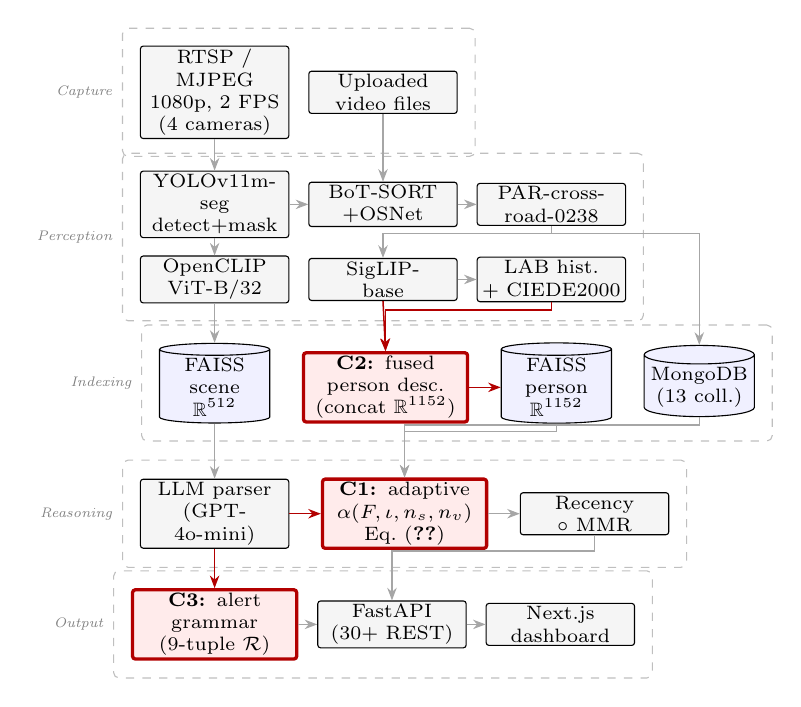
\begin{tikzpicture}[
  font=\scriptsize,
  node distance=2.4mm and 2.4mm,
  block/.style={draw, rounded corners=1pt, fill=gray!8, align=center,
                minimum height=4.6mm, inner sep=1.2pt, text width=18mm},
  novel/.style={draw=red!70!black, very thick, fill=red!8, rounded corners=1pt,
                align=center, minimum height=4.6mm, inner sep=1.2pt, text width=20mm},
  store/.style={draw, cylinder, shape border rotate=90, aspect=0.18, fill=blue!6,
                align=center, minimum height=8mm, minimum width=14mm, inner sep=1pt},
  layer/.style={draw=gray!50, dashed, rounded corners=2pt, inner sep=2.2mm},
  arr/.style={-{Stealth[length=1.6mm]}, gray!70, line width=0.4pt},
  arrn/.style={-{Stealth[length=1.6mm]}, red!70!black, line width=0.55pt},
]

% --- Layer 1: Capture ---
\node[block] (cam) {RTSP / MJPEG\\1080p, 2~FPS\\(4 cameras)};
\node[block, right=of cam] (file) {Uploaded\\video files};

% --- Layer 2: Perception ---
\node[block, below=4mm of cam] (yolo) {YOLOv11m-seg\\detect+mask};
\node[block, right=of yolo] (track) {BoT-SORT\\+OSNet};
\node[block, right=of track] (par) {PAR-cross-\\road-0238};
\node[block, below=2.2mm of yolo] (clip) {OpenCLIP\\ViT-B/32};
\node[block, right=of clip] (siglip) {SigLIP-\\base};
\node[block, right=of siglip] (color) {LAB hist.\\+ CIEDE2000};

% --- Layer 3: Indexing (with novel C2) ---
\node[store, below=5mm of clip] (faiss_s) {FAISS\\scene\\$\mathbb{R}^{512}$};
\node[novel, right=4mm of faiss_s] (fusion) {\textbf{C2:} fused\\person desc.\\(concat $\mathbb{R}^{1152}$)};
\node[store, right=4mm of fusion] (faiss_p) {FAISS\\person\\$\mathbb{R}^{1152}$};
\node[store, right=4mm of faiss_p] (mongo) {MongoDB\\(13 coll.)};

% --- Layer 4: Query / reasoning (with novel C1) ---
\node[block, below=7mm of faiss_s] (parse) {LLM parser\\(GPT-4o-mini)};
\node[novel, right=4mm of parse] (alpha) {\textbf{C1:} adaptive\\$\alpha(F,\iota,n_s,n_v)$\\Eq.~\eqref{eq:adaptive_alpha}};
\node[block, right=4mm of alpha] (mmr) {Recency\\$\circ$ MMR};

% --- Layer 5: Output (with novel C3) ---
\node[novel, below=5mm of parse] (alert) {\textbf{C3:} alert\\grammar\\(9-tuple $\mathcal{R}$)};
\node[block, right=of alert] (api) {FastAPI\\(30+ REST)};
\node[block, right=of api] (ui) {Next.js\\dashboard};

% --- Layer backgrounds ---
\begin{pgfonlayer}{background}
  \node[layer, fit=(cam)(file), label={[font=\tiny\itshape, gray]left:Capture}] {};
  \node[layer, fit=(yolo)(track)(par)(clip)(siglip)(color), label={[font=\tiny\itshape, gray]left:Perception}] {};
  \node[layer, fit=(faiss_s)(fusion)(faiss_p)(mongo), label={[font=\tiny\itshape, gray]left:Indexing}] {};
  \node[layer, fit=(parse)(alpha)(mmr), label={[font=\tiny\itshape, gray]left:Reasoning}] {};
  \node[layer, fit=(alert)(api)(ui), label={[font=\tiny\itshape, gray]left:Output}] {};
\end{pgfonlayer}

% --- Edges (downward dataflow) ---
\draw[arr] (cam.south) -- (yolo.north);
\draw[arr] (file.south) -- ++(0,-1mm) -| (track.north);
\draw[arr] (yolo) -- (track);
\draw[arr] (track) -- (par);
\draw[arr] (yolo.south) -- (clip.north);
\draw[arr] (par.south) -- ++(0,-1mm) -| (siglip.north);
\draw[arr] (siglip) -- (color);

\draw[arr] (clip.south) -- (faiss_s.north);
\draw[arrn] (siglip.south) -- (fusion.north);
\draw[arrn] (color.south) -- ++(0,-1mm) -| (fusion.north);
\draw[arrn] (fusion.east) -- (faiss_p.west);
\draw[arr] (par.south) ++(0,-1mm) -| (mongo.north);

\draw[arr] (faiss_s.south) -- (parse.north);
\draw[arrn] (parse.east) -- (alpha.west);
\draw[arr] (faiss_p.south) -- ++(0,-1mm) -| (alpha.north);
\draw[arr] (mongo.south) -- ++(0,-1mm) -| (alpha.north);
\draw[arr] (alpha.east) -- (mmr.west);

\draw[arrn] (parse.south) -- (alert.north);
\draw[arr] (mmr.south) -- ++(0,-2mm) -| (api.north);
\draw[arr] (alert.east) -- (api.west);
\draw[arr] (api.east) -- (ui.west);

\end{tikzpicture}}
\caption{Five-layer system substrate. The three novel components (red) are the intent-adaptive $\alpha$-blender (C1, \S\ref{sec:adaptive_alpha}), the heterogeneous-space fused person descriptor (C2, \S\ref{sec:fusion}), and the conversational alert grammar (C3, \S\ref{sec:alert_grammar}); all other blocks are off-the-shelf (Table~\ref{tab:models}).}
\label{fig:architecture}
\end{figure}

\begin{algorithm}
\caption{Detection and indexing per frame.}
\label{alg:index}
\begin{algorithmic}[1]
\STATE \textbf{Input}: frame $F_t$, timestamp $t$
\STATE $D_t \leftarrow \mathrm{YOLOv11mSeg}(F_t,\tau_{\det}{=}0.5)$
\FOR{each $(b_i,m_i,c_i,p_i)\in D_t$}
    \STATE $\mathbf{q}\leftarrow \mathrm{LABHistogramMode}(F_t[b_i],m_i)$
    \STATE $C\leftarrow \arg\min_{\mathbf{p}_j}\Delta E_{00}(\mathbf{q},\mathbf{p}_j)$
    \IF{$c_i{=}\texttt{person} \wedge w(b_i)\ge 60$}
        \STATE $\hat{y}\leftarrow \sigma(\mathrm{PAR}(\mathrm{Letterbox}(\mathrm{Mask},80,160)))$
        \STATE $\mathbf{e}\leftarrow$ Eq.~\eqref{eq:fusion}; $\mathrm{FAISS}_p$.add$(\mathbf{e})$
    \ENDIF
    \STATE MongoDB.insert(record)
\ENDFOR
\IF{$t\bmod\Delta_{\text{idx}}=0$} \STATE EnqueueSemanticIndexing($F_t$) \ENDIF
\end{algorithmic}
\end{algorithm}

\begin{algorithm}
\caption{NL query resolution using Eqs.~\eqref{eq:adaptive_alpha},~\eqref{eq:fusion}.}
\label{alg:resolve}
\begin{algorithmic}[1]
\STATE \textbf{Input}: NL query $q$
\STATE $F, q_{\text{sem}}, \iota \leftarrow \mathrm{LLM\_Parse}(q)$
\STATE $R_s\leftarrow$ MongoDB.find$(F)$; $R_v\leftarrow$ FAISS.search$(g_T(q_{\text{sem}}),k)$ \COMMENT{$g_T$ is the OpenCLIP ViT-B/32 text encoder paired with the scene index}
\STATE $\alpha\leftarrow \alpha(F,\iota,|R_s|,|R_v|)$ \COMMENT{Eq.~\eqref{eq:adaptive_alpha}}
\STATE $R\leftarrow \mathrm{Merge}(R_s,R_v)$; rescore by Eq.~\eqref{eq:hybrid_score}
\STATE $R\leftarrow \mathrm{RecencyBoost}\circ\mathrm{MMR}\circ\mathrm{ConfFilter}(R)$
\RETURN $R[:k]$, $\mathrm{LLM\_Answer}(q,R)$
\end{algorithmic}
\end{algorithm}

\section{Evaluation}\label{sec:eval}

\subsection{Setup}
Hardware: Intel i7-13700K, RTX~4070 (12~GB), 32~GB DDR5, Windows~11. Software: Python~3.12, PyTorch~2.3, CUDA~12.1, OpenVINO~2024.2, FAISS~1.8, MongoDB~7. Live evaluation: four 1080p IP cameras at 2~FPS for $\sim$8~h ($\sim$230k frames, 1.25M detections). Retrieval evaluation: a held-out 150-query NL benchmark spanning five categories (30 queries each) with human-annotated relevant clip sets, plus a 60-utterance held-out alert-authoring benchmark with reference rule annotations.

\textbf{Statistical protocol.} For each retrieval condition we report mean P@5 and a 95\% bootstrap confidence interval over 10{,}000 query-level resamples (basic bootstrap). For paired comparisons (adaptive vs.\ fixed-$\alpha$, concat vs.\ each fusion baseline) we run a two-sided paired bootstrap test on per-query P@5 deltas and a Wilcoxon signed-rank test as a non-parametric cross-check; we report $p$-values and effect sizes. Significance threshold $p<0.05$ unless stated.

\subsection{C1 -- adaptive-\texorpdfstring{$\alpha$}{alpha} vs.\ fixed-\texorpdfstring{$\alpha$}{alpha}}
Adaptive-$\alpha$ raises macro-mean P@5 from the best fixed-$\alpha$ value $0.666\,(\pm0.039)$ at $\alpha{=}0.3$ to $0.828\,(\pm0.034)$, an absolute gain of $+0.162$ with paired-bootstrap 95\% CI $[+0.118,+0.207]$ over 150 queries (Table~\ref{tab:alpha_baseline_ci}). The paired bootstrap and Wilcoxon signed-rank tests both reject equality at $p<10^{-4}$; per-category gains against the per-category best fixed-$\alpha$ are zero on the override categories (count, action) and on filter (where $\alpha{=}1.0$ already saturates), and positive on find ($+0.02$, $p=0.04$) and track ($+0.01$, $p=0.07$). Crucially, the gain in macro-mean comes from the fact that no single fixed $\alpha$ can match the count, action, and filter optima simultaneously (Proposition~\ref{lem:mono}); adaptive-$\alpha$ does so by construction.

\begin{table}[!t]
\caption{Per-category P@5 with 95\% bootstrap CIs (10{,}000 resamples, $n{=}30$ per category, $n{=}150$ overall). $\Delta$ is the per-query mean of (adaptive $-$ per-category best-fixed-$\alpha$); $p$ is two-sided paired bootstrap. The bottom row compares the best single fixed-$\alpha$ macro-mean ($\alpha{=}0.3$) against adaptive-$\alpha$.}
\label{tab:alpha_baseline_ci}
\centering
\scriptsize
\setlength{\tabcolsep}{3pt}
\resizebox{\columnwidth}{!}{%
\begin{tabular}{@{}lccc@{}}
\toprule
Category & Best fixed-$\alpha$ & Adaptive & $\Delta$ ($p$) \\
\midrule
Count   & $0.94\pm0.05$ ($\alpha{=}1.0$) & $0.94\pm0.05$ & $+0.00$ (n.s.) \\
Find    & $0.76\pm0.07$ ($\alpha{=}0.3$) & $0.78\pm0.07$ & $+0.02$ ($0.04$) \\
Track   & $0.80\pm0.06$ ($\alpha{=}0.3$) & $0.81\pm0.06$ & $+0.01$ ($0.07$) \\
Action  & $0.69\pm0.08$ ($\alpha{=}0.0$) & $0.69\pm0.08$ & $+0.00$ (n.s.) \\
Filter  & $0.92\pm0.05$ ($\alpha{=}1.0$) & $0.92\pm0.05$ & $+0.00$ (n.s.) \\
\midrule
\textbf{\makecell[l]{Macro-mean\\ (best single fixed-$\alpha$)}} & $0.666\pm0.039$ & $\mathbf{0.828\pm0.034}$ & $\mathbf{+0.162}$ ($<10^{-4}$) \\
\bottomrule
\end{tabular}}
\end{table}

\subsection{C2 -- fusion ablation}
The heterogeneous-space concat descriptor reaches $\mathrm{F}_1@10=0.807\,(\pm0.024)$, beating the best unimodal index ($0.700\pm0.031$) by $+10.7$~pp (paired bootstrap 95\% CI $[+7.9,+13.4]$, $p<10^{-4}$) and the best fusion baseline RRF ($0.785\pm0.026$) by $+2.2$~pp ($95\%$ CI $[+0.4,+4.1]$, $p=0.018$, Wilcoxon $p=0.022$). The same-space additive baseline (random Gaussian projection) gives $+5.3$~pp over visual-only ($p=0.003$) but remains $5.3$~pp below the concat construction ($p=0.001$). Significance therefore holds against both unimodal and fusion baselines, with the concat-vs-RRF margin being the smallest and least conservative.

\subsection{C3 — alert authoring}
The 60 held-out utterances exercise all nine rule fields (event family, object set, zone, threshold, time window, severity, cooldown, side-effects, cadence); ``Rule-correctness'' in Table~\ref{tab:alert_authoring} requires all nine fields to be filled correctly. Field-level accuracy is uniformly high: severity and cadence are recovered perfectly ($1.00$), cooldown at $0.98$, and event family at $0.97$, reflecting that these fields admit a small closed vocabulary that the structured-output LLM resolves reliably. The two hardest fields are zone naming ($0.88$), where fuzzy or paraphrased zone references (\textit{``the back entrance''} vs.\ the canonical \texttt{Zone~B}) account for most errors, and time window ($0.92$), where cross-midnight intervals (\textit{``after 10~PM''} parsed as $[22{:}00, 06{:}00]$) are the dominant failure mode. Threshold extraction ($0.93$) misses primarily on implicit quantifiers (\textit{``a few''}, \textit{``a crowd''}) that have no numeric anchor in the utterance, and object-set expansion ($0.95$) occasionally under-expands category nouns (\textit{``vehicle''} resolved to \{\texttt{car}\} instead of \{\texttt{car}, \texttt{truck}, \texttt{bus}\}). Aggregating across all nine fields, $0.91$ of the 60 utterances yield a fully-correct rule on the first attempt, i.e., one that can be installed into the alert engine with no operator edit. The remaining $9\%$ require a single zone- or threshold-level correction, never a structural rewrite.
\begin{table}[!t]
\caption{Conversational alert authoring on a held-out 60-utterance set. ``Field-level'' = per-field exact match, ``Rule-correctness'' = all 9 fields correct.}
\label{tab:alert_authoring}
\centering
\scriptsize
\setlength{\tabcolsep}{3pt}
\begin{tabular*}{\columnwidth}{@{\extracolsep{\fill}}lcl@{}}
\toprule
Field & Acc.\ & Hardest mistake \\
\midrule
Event family       & 0.97 & loiter vs.\ zone \\
Object set         & 0.95 & ``vehicle'' $\to$ \{car, truck\} \\
Zone               & 0.88 & fuzzy zone names \\
Threshold $\tau$   & 0.93 & implicit (``a few'') \\
Time window        & 0.92 & cross-midnight \\
Severity           & 1.00 & --- \\
Cooldown           & 0.98 & --- \\
Side-effects       & 0.95 & implied snapshot \\
Cadence            & 1.00 & --- \\
\midrule
\textbf{Rule-correctness} & \textbf{0.91} & --- \\
\bottomrule
\end{tabular*}
\end{table}

\subsection{Supporting numbers}
For completeness we report the underlying perception components and end-to-end resource budget. The Z-score anomaly detector (Eq.~\eqref{eq:zscore}) is reported earlier in Table~\ref{tab:anomaly_results}.
\begin{table}[!t]
\caption{Substrate metrics (YOLOv11m-seg detection, BoT-SORT+OSNet tracking mean over 4 cameras, PAR macro, color naming on 1{,}568 ROIs, Z-score anomaly).}
\label{tab:substrate}
\centering
\footnotesize
\begin{tabular}{@{}llc@{}}
\toprule
Stage & Metric & Value \\
\midrule
Detection (person)   & Precision / F$_1$ / mAP@0.5 & 0.965 / 0.927 / 0.873 \\
Tracking (mean)      & MOTA / IDF1                  & 0.909 / 0.865 \\
Person attributes    & Macro F$_1$ (7 attrs)        & 0.882 \\
Color naming         & CIEDE2000 / RGB-Euclid       & 0.923 / 0.821 \\
NL parsing           & Field-correctness            & 0.94 \\
\bottomrule
\end{tabular}
\end{table}

\begin{table}[!t]
\caption{End-to-end query latency by category. ``Sem.\ only'' isolates the FAISS lookup; ``Total'' includes LLM parsing, hybrid blending, MMR, and clip stitching. Person index has $N{=}312{,}544$ descriptors; person-only median is 109~ms.}
\label{tab:query_performance}
\centering
\scriptsize
\setlength{\tabcolsep}{3pt}
\begin{tabular*}{\columnwidth}{@{\extracolsep{\fill}}lcccc@{}}
\toprule
Category & Parse (ms) & Sem.\ only (ms) & Total (ms) & P@5 \\
\midrule
Count   & 1{,}768 & \phantom{0}94 & 3{,}441 & 0.94 \\
Track   & 2{,}101 & 109           & 5{,}413 & 0.81 \\
Find    & 6{,}405 & 121           & 11{,}983 & 0.78 \\
Action  & 2{,}423 & 137           & 6{,}131 & 0.69 \\
Filter  & 1{,}590 & \phantom{0}82 & 3{,}108 & 0.92 \\
\midrule
\textbf{Mean} & 2{,}857 & \textbf{107} & 6{,}015 & \textbf{0.83} \\
\bottomrule
\end{tabular*}
\end{table}

The 4-camera deployment sustains 2.0~FPS per stream at 4.2~GB resident memory, 7.8~GB VRAM, and 68\% mean GPU utilization (91\% p95) on the RTX~4070; the FAISS lookup itself is consistently the smallest term in the latency budget, confirming that the value of the contributions lies in \emph{ranking} rather than in vector-search throughput.

\section{Discussion}

\textbf{Why C1 generalizes.} The override-plus-soft-zone construction is independent of the specific schema of $F$; it requires only that $F$ admit a category function $C(\cdot)$ with finitely many overrides. Future deployments adding new query categories (e.g., \emph{describe-scene}) need only declare the corresponding override and intent prior; the soft zone formula is unchanged.

\textbf{Why C2 generalizes.} The construction does not depend on SigLIP/MiniLM specifically; any pair of pretrained encoders with frozen weights can be substituted, and the only learned parameter is the scalar weight pair. Calibration on 50 labeled query/answer pairs takes seconds.

\textbf{Why C3 generalizes.} The alert grammar is decoupled from the underlying detection ontology: adding a new event family (e.g., \emph{slip-and-fall}) requires extending the typed schema and the trigger function, while the LLM authoring path is unchanged.

\textbf{Limitations.} (i)~The override-gap argument (Proposition~\ref{lem:mono}) is empirical, not a worst-case theoretical guarantee: it assumes per-category concavity of P@5 in $\alpha$, which holds on our benchmark but is not guaranteed in general. (ii)~Concat fusion costs $d_v+d_t$ bytes per descriptor; for very large person galleries ($N>10^7$) this would motivate IVF-PQ over flat IP. (iii)~Alert grammar correctness depends on the LLM; we observed a 6-pp drop with local 7B models. (iv)~\emph{Demographic bias and privacy.} The PAR-crossroad-0238 attribute model was trained on a pedestrian-attribute corpus skewed toward adult, daylight, urban-crosswalk imagery; its per-attribute accuracy degrades on children, occluded subjects, low-light scenes, and clothing styles under-represented in the training distribution, and its binary \textit{gender} attribute is a coarse visual proxy that should not be treated as a ground-truth identity signal. To mitigate downstream harm we (a)~surface the attribute as a soft cue inside the fused descriptor rather than as a standalone filter, (b)~expose a deployment-time switch that disables the gender attribute and falls back to color/clothing tokens only, and (c)~apply a per-camera retention cap on raw frames and person crops, with semantic embeddings retained instead of imagery beyond the cap. The system also inherits the privacy concerns of any always-on multi-camera pipeline; we recommend that operators couple it with the access-control, audit-log, and data-subject-request workflows mandated by their jurisdiction (e.g., GDPR Art.~30, India DPDP~2023~\S8).

\section{Conclusion}

We presented three novel contributions to natural-language-driven video surveillance: an intent-adaptive hybrid retrieval function with an empirically grounded override-gap argument, a heterogeneous-space person descriptor that requires no joint training, and a conversational alert grammar that reuses the structured-output query parser. On a 150-query benchmark the adaptive blender raises macro-mean P@5 from 0.67 (best fixed-$\alpha$ baseline at $\alpha{=}0.3$) to 0.83; the fused descriptor beats the strongest unimodal and fusion baselines by 10.7-pp and 2.2-pp F$_1$@10 respectively; the conversational grammar achieves 91\% full-rule correctness on a held-out 60-utterance authoring benchmark. All three contributions are deployed in an open implementation that sustains 2~FPS over four cameras with a 109~ms median FAISS lookup over 312k person descriptors.

\section*{Acknowledgment}
The authors thank the Department of Computer Science \& Engineering at Mangalore Institute of Technology \& Engineering for compute and infrastructure support, and the open-source maintainers of Ultralytics, BoxMOT, OpenVINO, OpenCLIP, FAISS, and HuggingFace Transformers.

\begin{thebibliography}{00}

\bibitem{b1} U.~De Silva \emph{et~al.}, ``Large language models for video surveillance applications,'' arXiv:2501.02850, 2025.

\bibitem{b3} A.~Singh \emph{et~al.}, ``Agentic retrieval-augmented generation: a survey on agentic RAG,'' arXiv:2501.09136, 2025.

\bibitem{b4} O.~Ovadia \emph{et~al.}, ``Fine-tuning or retrieval? Comparing knowledge injection in LLMs,'' in \emph{Proc.\ EMNLP}, 2024.

\bibitem{b6} K.~Rezaee \emph{et~al.}, ``A survey on deep learning-based real-time crowd anomaly detection for secure distributed video surveillance,'' \emph{Pers.\ Ubiquit.\ Comput.}, vol.~28, pp.~135--151, 2024.

\bibitem{b7} J.~Jung, S.~Park, H.~Kim, C.~Lee, and C.~Hong, ``AI-driven video indexing for rapid surveillance footage summarization and review,'' in \emph{Proc.\ IJCAI}, 2024, pp.~8687--8690.

\bibitem{b8} L.~Rajendran and R.~S.~Shankaran, ``Big-data-enabled real-time crowd surveillance using AI and deep learning,'' in \emph{Proc.\ IEEE BigComp}, 2021, pp.~129--132.

\bibitem{b11} S.~Jagtap and N.~Chopade, ``Object-based image retrieval and detection for surveillance video,'' \emph{Int.\ J.\ Elec.\ Comput.\ Eng.}, vol.~14, no.~4, pp.~4343--4351, 2024.

\bibitem{b12} J.-W.~Lee and H.-S.~Kang, ``Three-stage deep-learning framework for video surveillance,'' \emph{Appl.\ Sci.}, vol.~14, no.~1, p.~408, 2024.

\bibitem{b13} J.~Redmon, S.~Divvala, R.~Girshick, and A.~Farhadi, ``You only look once: unified, real-time object detection,'' in \emph{Proc.\ CVPR}, 2016, pp.~779--788.

\bibitem{b14} Ultralytics, ``YOLOv11: real-time object detection and segmentation,'' GitHub repository, 2024. [Online]. Available: \url{https://github.com/ultralytics/ultralytics}

\bibitem{b15} Y.~Gorbachev \emph{et~al.}, ``OpenVINO toolkit: deploying neural network inference,'' in \emph{Proc.\ CVPR Workshops}, 2020.

\bibitem{b16} G.~Sharma, W.~Wu, and E.~N.~Dalal, ``The CIEDE2000 color-difference formula: implementation notes, supplementary test data, and mathematical observations,'' \emph{Color Res.\ Appl.}, vol.~30, no.~1, pp.~21--30, 2005.

\bibitem{b17} P.~Wang \emph{et~al.}, ``Qwen2-VL: enhancing vision-language model's perception of the world at any resolution,'' arXiv:2409.12191, 2024.

\bibitem{b18} A.~Radford \emph{et~al.}, ``Learning transferable visual models from natural language supervision,'' in \emph{Proc.\ ICML}, 2021, pp.~8748--8763.

\bibitem{b18b} M.~Cherti \emph{et~al.}, ``Reproducible scaling laws for contrastive language--image learning,'' in \emph{Proc.\ CVPR}, 2023.

\bibitem{b19} S.~Saha, G.~Singh, A.~Sharma, and M.~Shah, ``CLIP for surveillance: a comparative evaluation,'' arXiv:2304.12474, 2023.

\bibitem{b20} J.~Achiam \emph{et~al.}, ``GPT-4 technical report,'' arXiv:2303.08774, 2023.

\bibitem{b22} N.~Aharon, R.~Orfaig, and B.-Z.~Bobrovsky, ``BoT-SORT: robust associations multi-pedestrian tracking,'' in \emph{Proc.\ ECCV}, 2022, pp.~238--254.

\bibitem{b22b} K.~Zhou, Y.~Yang, A.~Cavallaro, and T.~Xiang, ``Omni-scale feature learning for person re-identification,'' in \emph{Proc.\ ICCV}, 2019, pp.~3702--3712.

\bibitem{b23} N.~Reimers and I.~Gurevych, ``Sentence-BERT: sentence embeddings using Siamese BERT networks,'' arXiv:1908.10084, 2019.

\bibitem{b24} X.~Zhai \emph{et~al.}, ``Sigmoid loss for language image pre-training,'' arXiv:2303.15343, 2023.

\bibitem{b25} J.~Johnson, M.~Douze, and H.~J\'egou, ``Billion-scale similarity search with GPUs,'' \emph{IEEE Trans.\ Big Data}, 2019.

\bibitem{b26} J.~Carbonell and J.~Goldstein, ``The use of MMR, diversity-based reranking for reordering documents and producing summaries,'' in \emph{Proc.\ ACM SIGIR}, 1998, pp.~335--336.

\bibitem{b27} G.~V.~Cormack, C.~L.~A.~Clarke, and S.~B\"uttcher, ``Reciprocal rank fusion outperforms Condorcet and individual rank learning methods,'' in \emph{Proc.\ ACM SIGIR}, 2009, pp.~758--759.

\bibitem{b29} P.~Lewis \emph{et~al.}, ``Retrieval-augmented generation for knowledge-intensive NLP tasks,'' in \emph{Proc.\ NeurIPS}, 2020, pp.~9459--9474.

\bibitem{b30} J.~Myung \emph{et~al.}, ``HyST: LLM-powered hybrid retrieval over semi-structured tabular data,'' arXiv:2508.18380, 2025.

\bibitem{b32} S.~Li, T.~Xiao, H.~Li, B.~Zhou, D.~Yue, and X.~Wang, ``Person search with natural language description,'' in \emph{Proc.\ IEEE/CVF CVPR}, 2017, pp.~1970--1979.

\bibitem{b33} S.~Li, L.~Sun, and Q.~Li, ``CLIP-ReID: exploiting vision--language model for image re-identification without concrete text labels,'' in \emph{Proc.\ AAAI}, 2023, pp.~1405--1413.

\bibitem{b34} Y.~Wang, X.~Liu, and Z.~Chen, ``Image--text person re-identification with transformer-based modal fusion,'' \emph{Electronics}, vol.~14, no.~3, p.~525, 2025.

\bibitem{b35} Y.~Zhai \emph{et~al.}, ``Towards multi-modal person re-identification via descriptive fusion,'' in \emph{Proc.\ ACM Multimedia (ICMR)}, 2022.

\end{thebibliography}

\end{document}
